\bookchapter{The perception pipeline}\label{ch:ctl6}

\section*{Explanation}
The robot sees a ball. What the neural network of Chapter~\ref{ch:ai4} delivers is a rectangle in an image: ``ball, pixels $(750\dots810,\ 470\dots530)$, confidence $0.91$''. What the behaviour needs is a statement about the world: ``the ball is $1.2$\,m in front of me, $0.3$\,m to the left, and rolling away at $0.4$\,m/s''. Everything that happens in between is the \textbf{perception pipeline}. Its stages are the topic of this chapter, and all the tools came earlier in the book: geometry (Part~\ref{part:math}), the Kalman filter (Chapter~\ref{ch:ctl3}), the orientation (Chapter~\ref{ch:ctl4}) and localisation (Chapter~\ref{ch:ctl5}).

\begin{center}
\begin{tikzpicture}[>={Stealth[length=2.2mm]},bx/.style={draw,thick,rounded corners=2pt,minimum width=2.15cm,minimum height=1.0cm,font=\scriptsize,align=center}]
 \node[bx,fill=gray!15] (cam) at (0,0) {camera\\ image + \textbf{time stamp}};
 \node[bx,fill=blue!10] (det) at (2.9,0) {detector\\ (network)};
 \node[bx,fill=yellow!20] (geo) at (5.8,0) {geometry\\ pixel $\to$ field};
 \node[bx,fill=orange!15] (trk) at (8.7,0) {tracking\\ (Kalman filter)};
 \node[bx,fill=green!10] (wm) at (11.6,0) {world model\\ $\to$ behaviour};
 \draw[->,thick] (cam)--(det); \draw[->,thick] (det)--(geo); \draw[->,thick] (geo)--(trk); \draw[->,thick] (trk)--(wm);
 \node[font=\scriptsize,below=0.9cm of geo,align=center] (pose) {camera pose: head joints,\\ trunk tilt (IMU), position (localisation)};
 \draw[->,thick] (pose)--(geo);
\end{tikzpicture}
\captionof{figure}{The stages between a camera image and the world model. The geometry stage needs the pose of the camera at the moment of the image.}
\end{center}

\section*{The camera as a pinhole}
A camera is described, to a good approximation, by the \textbf{pinhole model}: a point at the position $(X,Y,Z)$ in the camera frame ($X$ to the right, $Y$ down, $Z$ along the viewing direction) appears at the pixel
\[
u=c_x+f\,\frac{X}{Z},\qquad v=c_y+f\,\frac{Y}{Z}.
\]
The \textbf{focal length} $f$ in pixels and the \textbf{principal point} $(c_x,c_y)$ (usually near the centre of the image) are the \textbf{intrinsic parameters} of the camera. If the horizontal field of view is $\alpha$ and the image is $W$ pixels wide, then $f=\dfrac{W/2}{\tan(\alpha/2)}$. The intrinsic parameters are determined once, by photographing a checkerboard from different sides (the calibration functions of OpenCV, Chapter~\ref{ch:py10}). Lens distortion, which bends straight lines near the edges, is corrected first and ignored here.

In this chapter the example camera has an image of $1280\times720$ pixels and a field of view of $90^{\circ}$, so $f=640$ pixels and $(c_x,c_y)=(640,360)$; it is mounted $H=0.55$\,m above the ground and looks forward and downwards, \textbf{pitched} by $\varphi=25^{\circ}$. (All these numbers are assumptions of the example, not the data of any robot; the true values for the K1 are found by calibration.)

\begin{example}
A point is $0.3$\,m to the right, $0.1$\,m below the optical axis and $2.0$\,m in front of the camera: $(X,Y,Z)=(0.3,0.1,2.0)$. Then $u=640+640\cdot0.3/2=736$ and $v=360+640\cdot0.1/2=392$.
\end{example}

\section*{From a pixel to the ground}
A pixel does not determine a point in space but a \emph{ray}: everything on the line from the camera through the pixel. For a ball (or a foot, a line, a goal post) we know that it \emph{touches the ground}, and the ray meets the ground at one point only. Let $a=(u-c_x)/f$ and $b=(v-c_y)/f$ (the slope of the ray to the right and downwards). With the robot frame ($x$ forward, $y$ left, $z$ up), a camera at the height $H$ and the pitch $\varphi$, the ray hits the ground at
\[
x=H\,\frac{\cos\varphi-b\sin\varphi}{\sin\varphi+b\cos\varphi},\qquad
y=-H\,\frac{a}{\sin\varphi+b\cos\varphi}.
\]
The denominator is the sine of the angle between the ray and the horizontal; if it is $\le0$ the pixel lies on or above the horizon and does not see the ground. In the example the horizon is at the row $360-640\tan25^{\circ}=61.5$.

\begin{center}
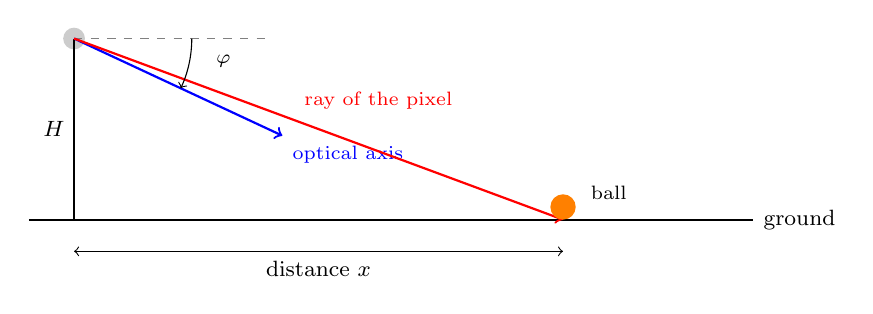
\begin{tikzpicture}[scale=1.15]
 \draw[thick] (-0.5,0)--(7.5,0) node[right,font=\footnotesize]{ground};
 \fill[gray!40] (0,2.0) circle (0.12); \draw[thick] (0,0)--(0,2.0);
 \node[font=\footnotesize,left] at (0,1.0) {$H$};
 \draw[dashed,gray] (0,2.0)--(2.2,2.0);
 \draw[->,thick,blue] (0,2.0)--(2.3,2.0-2.3*0.4663) node[below right,font=\scriptsize]{optical axis};
 \draw[->,thick,red] (0,2.0)--(5.4,0.0) node[above right,pos=0.45,font=\scriptsize]{ray of the pixel};
 \draw[->] (1.3,2.0) arc (0:-25:1.3); \node[font=\scriptsize] at (1.65,1.75) {$\varphi$};
 \fill[orange] (5.4,0.14) circle (0.14); \node[font=\scriptsize,right] at (5.6,0.3) {ball};
 \draw[<->] (0,-0.35)--(5.4,-0.35) node[midway,below,font=\footnotesize]{distance $x$};
\end{tikzpicture}
\captionof{figure}{Side view. The camera is $H$ above the ground and looks down by $\varphi$; the ray through the pixel meets the ground in the point where the ball touches it.}
\end{center}

\begin{example}
The ball is detected at $(u,v)=(800,500)$. Then $a=0.25$, $b=0.21875$; $\sin25^{\circ}=0.4226$, $\cos25^{\circ}=0.9063$. The denominator is $0.4226+0.21875\cdot0.9063=0.6209$ and the numerator $0.9063-0.21875\cdot0.4226=0.8139$, so $x=0.55\cdot0.8139/0.6209=0.721$\,m and $y=-0.55\cdot0.25/0.6209=-0.221$\,m: the ball is $0.72$\,m ahead and $0.22$\,m to the \emph{right} ($y$ is positive to the left).
\end{example}

\subsection*{Far away, small errors become large errors}
Look at the way in which the image row $v$ is translated into a distance:
\begin{center}
\begin{tikzpicture}
\begin{axis}[width=0.8\linewidth,height=5cm,xlabel={image row $v$ of the ground contact point},ylabel={distance $x$ (m)},xmin=100,xmax=440,ymin=0,ymax=12,grid=both,x dir=reverse]
 \addplot[blue,very thick] table[x=v,y=x] {chapters/part09_control_perception/06_the_perception_pipeline/dist.dat};
 \addplot[red,dashed] coordinates {(61.5,0)(61.5,12)};
\end{axis}
\end{tikzpicture}
\captionof{figure}{The distance as a function of the pixel row (camera as in the text). Near the robot (large $v$) one pixel is a few millimetres; near the horizon (red, the row $61.5$) one pixel means metres.}
\end{center}
One pixel of error in the row corresponds to $3.7$\,mm at $1$\,m, $12$\,mm at $2$\,m, $42$\,mm at $4$\,m and $91$\,mm at $6$\,m: the sensitivity grows with the \emph{square} of the distance. A precise detection in the image is thus not the largest problem at long distance; the pitch of the camera is. If the pitch is wrong by $1^{\circ}$ (because the head is not exactly where the joint angles say, or the trunk tilt is not exact, Chapter~\ref{ch:ctl4}), the error at $2$\,m is $-0.13/+0.15$\,m, at $4$\,m already $-0.46/+0.59$\,m, and at $6$\,m $-0.97/+1.42$\,m. The camera pose is part of the measurement.

\section*{A second estimate: the size of the ball}
The ball has a known diameter $D$ (say $0.14$\,m). If it appears with the width $w$ pixels, then by the pinhole formula $w=fD/\text{range}$, and the straight-line distance from the camera is $\text{range}=fD/w$; the ground distance is $\sqrt{\text{range}^2-H^2}$. This method does \emph{not} depend on the pitch of the camera, but a width error of a few pixels is large for a small ball ($w=22$ pixels at $4$\,m).

The two estimates are independent, with different errors, and this is the Kalman situation of Chapter~\ref{ch:ctl3}: weigh them with the inverse of their variances.
\begin{example}
Ground-plane method: $4.1$\,m with a standard deviation of $0.5$\,m. Size method: $3.7$\,m with $0.4$\,m. The weights are $1/0.25=4$ and $1/0.16=6.25$, so
\[
\hat d=\frac{4\cdot4.1+6.25\cdot3.7}{4+6.25}=3.86\ \text{m},\qquad \sigma=\sqrt{\frac{1}{10.25}}=0.31\ \text{m}.
\]
The combination is better than each one alone.
\end{example}
A Monte Carlo test of the example camera ($20\,000$ trials per distance, with random errors of $2$ pixels in the row, $3$ pixels in the width and $0.7^{\circ}$ in the pitch, all assumed) gives the root-mean-square errors:
\begin{center}\small
\begin{tabular}{r c c c}
\hline
true distance & ground-plane method & size method & weighted combination\\\hline
1\,m & 0.030\,m & 0.050\,m & 0.025\,m\\
2\,m & 0.100\,m & 0.152\,m & 0.084\,m\\
3\,m & 0.218\,m & 0.333\,m & 0.182\,m\\
4\,m & 0.388\,m & 0.606\,m & 0.329\,m\\
6\,m & 0.905\,m & 1.523\,m & 0.787\,m\\\hline
\end{tabular}
\end{center}
(The weights were set from the errors of each method at that distance; in a real system they come from the estimated uncertainties.) Without the pitch error the ground-plane method would have $0.085$\,m at $4$\,m and the size method would be hopelessly worse: which of the two is better depends on which error is larger, and \emph{that is a statement about your robot}, to be measured.

\section*{Time: the image is old}
Between the moment at which the sensor takes the picture and the moment at which the detection is available, time passes: exposure and readout, transfer, the network (Chapter~\ref{ch:ai4}), the queue before the next processing step. Typical numbers for such a chain are tens of milliseconds, and a long pipeline reaches $100$\,ms. In this time a walking robot moves and its head turns. If the geometry stage uses the camera pose of \emph{now}, the ball appears at the wrong place.

\begin{example}
The robot turns at $60^{\circ}$/s and the detection arrives $0.1$\,s late. The heading has changed by $6^{\circ}$, and a ball at $4$\,m seems to be $4\tan6^{\circ}=0.42$\,m to the side of its true position.
\end{example}

The remedy is simple, and every vision system has it: \textbf{time stamps}. The camera attaches the time of exposure to the image; the pipeline carries it along with the detection; and the geometry stage uses the \emph{pose at that time}, found in a short buffer of past poses (head angles, trunk orientation, position), interpolated between the stored entries. The same applies to the Kalman filter: a delayed measurement is applied at its own time, or the filter is predicted forward. In ROS (Part~\ref{part:ros}) the messages have a \verb!header.stamp! for this, and the transformation library keeps the buffer of poses.

\section*{Tracking the ball}
After the geometry stage the detections are points $(x,y)$ on the field, with noise, gaps (the ball is hidden) and false detections. The ball tracker is the Kalman filter of Chapter~\ref{ch:ctl3} for the state $(x,y,v_x,v_y)$, with the gate for outliers, the prediction through gaps and a model of the friction (the ball slows down, its speed reduces by a constant factor per second, and one measures this factor on the real field). Its velocity estimate allows the goalkeeper to decide to dive, and the striker to move to where the ball \emph{will be}.

\section*{In code}
Pixels to ground and back, and the size method, in Rust. The two directions are checked against each other: the result of one must reproduce the input of the other.
%rs:cam
\begin{verbatim}
struct Camera {
    f: f64,                 // focal length in pixels
    cx: f64,                // principal point (image centre)
    cy: f64,
    height: f64,            // height of the camera above the ground (m)
    pitch: f64,             // looking down by this angle (rad)
}

impl Camera {
    /// Pixel -> point on the ground (x forward, y left), in metres.
    /// None if the ray does not hit the ground (at or above the horizon).
    fn to_ground(&self, u: f64, v: f64) -> Option<(f64, f64)> {
        let a = (u - self.cx) / self.f;
        let b = (v - self.cy) / self.f;
        let den = self.pitch.sin() + b * self.pitch.cos();
        if den <= 1e-9 {
            return None;
        }
        let x = self.height * (self.pitch.cos() - b * self.pitch.sin()) / den;
        let y = -self.height * a / den;
        Some((x, y))
    }

    /// Point on the ground -> pixel (the opposite direction).
    fn to_pixel(&self, x: f64, y: f64) -> (f64, f64) {
        let (dx, dz) = (x, -self.height);
        let cam_x = -y;
        let cam_y = -self.pitch.sin() * dx - self.pitch.cos() * dz;
        let cam_z = self.pitch.cos() * dx - self.pitch.sin() * dz;
        (self.cx + self.f * cam_x / cam_z, self.cy + self.f * cam_y / cam_z)
    }

    /// Distance along the ground from the apparent width of a ball.
    fn distance_from_size(&self, ball: f64, width_px: f64) -> f64 {
        let range = self.f * ball / width_px;    // straight line to the ball
        (range * range - self.height * self.height).sqrt()
    }
}

fn main() {
    let cam = Camera { f: 640.0, cx: 640.0, cy: 360.0,
                       height: 0.55, pitch: 25f64.to_radians() };
    let (x, y) = cam.to_ground(800.0, 500.0).unwrap();
    println!("pixel (800, 500) -> x {x:.3} m, y {y:.3} m");
    let (u, v) = cam.to_pixel(x, y);
    println!("and back: ({u:.1}, {v:.1})");
    println!("horizon row: {:?}", cam.to_ground(640.0, 61.0));
    for d in [1.0, 2.0, 4.0, 6.0] {
        let (u, v) = cam.to_pixel(d, 0.0);
        let width = 640.0 * 0.14 / (d * d + 0.55 * 0.55_f64).sqrt();
        println!("{d} m: row {v:.1}, width {width:.1} px, \
                  from width {:.2} m", cam.distance_from_size(0.14, width));
        let _ = u;
    }
}
\end{verbatim}
prints
\begin{center}\small\ttfamily
\begin{tabular}{@{}l@{}}
pixel (800, 500) -> x 0.721 m, y -0.221 m\\
and back: (800.0, 500.0)\\
horizon row: None\\
1 m: row 402.6, width 78.5 px, from width 1.00 m\\
2 m: row 251.5, width 43.2 px, from width 2.00 m\\
4 m: row 162.2, width 22.2 px, from width 4.00 m\\
6 m: row 130.1, width 14.9 px, from width 6.00 m
\end{tabular}
\end{center}
The first line is the example of the text. The function returns \verb!None! for pixels that do not see the ground, so the case ``at the horizon'' cannot be forgotten by the caller (Chapter~\ref{ch:rust5}). The table shows how small the ball becomes: $15$ pixels wide at $6$\,m, which every detector must still find.

\begin{keyidea}[Where the errors come from]
Detection noise in the image, a wrong camera pitch or height, a time delay and a wrong robot pose each add to the error of the ball position. Measure each of them separately (move the ball to known marks on the field and compare), and spend your effort on the largest one. At long distance this is rarely the neural network.
\end{keyidea}

\begin{aibox}[Detection is not the end]
A network that finds the ball in $98\%$ of the images does not make a robot that plays well. The pipeline decides whether those detections become a good world model: with the right time, the right pose, the right uncertainty. When the debugging tool of the team shows the raw detections, the filtered ball and the field lines on one screen, errors in these stages become visible.
\end{aibox}

\section*{Practice problems}
\begin{enumerate}[label=\textbf{\thechapter.\arabic*}]
  \item An image is $1920$ pixels wide and the horizontal field of view is $70^{\circ}$. Compute the focal length in pixels.
  \item With $f=640$, $(c_x,c_y)=(640,360)$: where do the points $(X,Y,Z)=(0.3,\,0.1,\,2.0)$ and $(-0.5,\,0,\,1.0)$ appear in the image?
  \item For the camera of the chapter ($H=0.55$\,m, $\varphi=25^{\circ}$), where on the ground does the pixel $(640,300)$ lie? Which pixel row would you expect for a ball at $3$\,m, and what is the width of the ball ($0.14$\,m) there in pixels (use the straight-line range $\sqrt{3^2+0.55^2}$)?
  \item A ball ($D=0.14$\,m) appears $20$ pixels wide ($f=640$). What is the straight-line distance, and, for $H=0.55$\,m, the ground distance? How many metres does the result change if the width is measured as $19$ pixels?
  \item Combine the estimates $2.0$\,m ($\sigma=0.1$) and $2.3$\,m ($\sigma=0.3$) of the distance of an object. Compute the weights, the result and its standard deviation. Why is the result closer to the first estimate?
  \item The head turns at $90^{\circ}$/s and the detection is $80$\,ms old. How large is the angle error if the current head angle is used, and how large is the position error of a ball at $3$\,m?
  \item A camera at $H=0.55$\,m is pitched so that a ball $3$\,m ahead appears exactly in the centre of the image (the pitch is then the depression angle $\arctan(H/3)$). By how many centimetres does the computed distance change if the pitch is believed to be $1^{\circ}$ more, or $1^{\circ}$ less? (Use $d=H/\tan(\text{depression angle})$.)
  \item Why does a ball that is detected \emph{just below the horizon} give a nearly useless distance, even if the detection is perfect (one pixel error)? What would a good pipeline do with this detection?
  \item Write Python functions \verb!to_ground(u,v)! and \verb!to_pixel(x,y)! for the camera of the chapter and check the round trip for a grid of $(x,y)$ with $x=0.5\dots6$\,m and $y=-2\dots2$\,m: print the largest error.
  \item[\textbf{\thechapter.10}$\star$] Write a Rust program with a buffer of the past headings of the robot (time stamp and angle, one entry every $10$\,ms, the robot turns at $60^{\circ}$/s), with a function that returns the heading at any time by linear interpolation. A ball stands at the field position $(3,\,0.5)$ and the robot is at the origin. The image is taken at $t_0=1.000$\,s; the detection is processed at $t_0+0.1$\,s. Compute the ball position in the field frame (a) with the current heading, (b) with the interpolated heading at $t_0$. Report both errors.
\end{enumerate}
